% Copyright (c) 2026 Islam Ibrahim. All rights reserved.

\documentclass[tikz,border=10pt]{standalone}
\usepackage[T1]{fontenc}
\usepackage{amsmath}
\usepackage{tikz}
\usetikzlibrary{arrows.meta,decorations.pathreplacing,positioning,calc}

\begin{document}
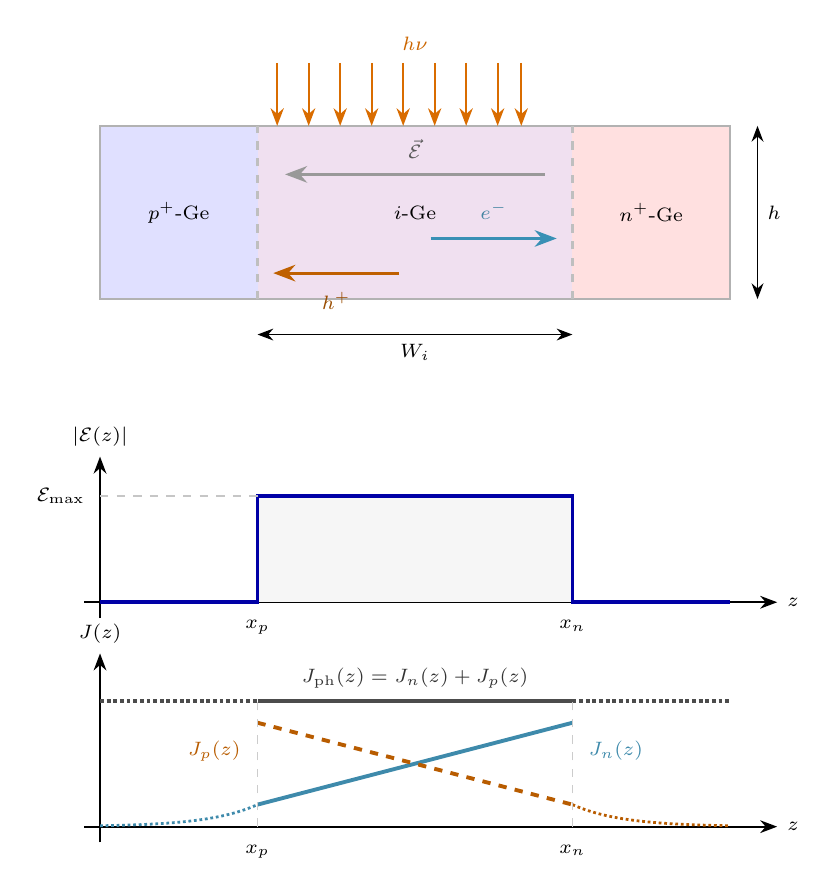
\begin{tikzpicture}[
  font=\small\rmfamily,
  >=Stealth,
  lbl/.style  = {font=\scriptsize\rmfamily},
  ax/.style   = {line width=0.7pt, ->},
  seg/.style  = {line width=1.4pt},
  thk/.style  = {line width=0.8pt},
]

\def\pW{2.0} \def\iW{4.0} \def\nW{2.0}
\def\TW{\pW+\iW+\nW}
\def\pH{2.2}
\def\rowgap{0.8}
\def\yA{11.0}

\fill[blue!12]   (0,\yA)       rectangle (\pW,     \yA+\pH);
\fill[violet!12] (\pW,\yA)     rectangle (\pW+\iW, \yA+\pH);
\fill[red!12]    (\pW+\iW,\yA) rectangle (\TW,     \yA+\pH);

\draw[thk,gray!60] (0,\yA) rectangle (\TW,\yA+\pH);
\draw[thk,gray!50,dashed]
  (\pW,\yA)--(\pW,\yA+\pH)
  (\pW+\iW,\yA)--(\pW+\iW,\yA+\pH);

\node[lbl] at (\pW/2,         \yA+\pH*0.50) {$p^{+}$-Ge};
\node[lbl] at (\pW+\iW/2,     \yA+\pH*0.50) {$i$-Ge};
\node[lbl] at (\pW+\iW+\nW/2, \yA+\pH*0.50) {$n^{+}$-Ge};

\draw[<->,line width=0.6pt]
  (\TW+0.35, \yA) -- (\TW+0.35, \yA+\pH)
  node[midway,right,lbl]{$h$};

\draw[<->,line width=0.6pt]
  (\pW, \yA-0.45) -- (\pW+\iW, \yA-0.45)
  node[midway,below,lbl]{$W_{i}$};

\def\aH{0.8}
\foreach \xp in {0.25,0.65,1.05,1.45,1.85,2.25,2.65,3.05,3.35}{
  \draw[orange!85!black,line width=0.75pt,->]
    ({\pW+\xp},\yA+\pH+\aH) -- ({\pW+\xp},\yA+\pH);
}
\node[lbl,orange!80!black,above=1pt] at (\pW+\iW/2,\yA+\pH+\aH)
  {$h\nu$};

\draw[line width=1.1pt,->,gray!80]
  (\pW+\iW-0.35, \yA+\pH*0.72) -- (\pW+0.35, \yA+\pH*0.72)
  node[midway,above=2pt,lbl,gray!70!black]{$\vec{\mathcal{E}}$};

\draw[cyan!70!black,line width=1.1pt,->]
  (\pW+\iW/2+0.2, \yA+\pH*0.35) -- (\pW+\iW-0.2, \yA+\pH*0.35)
  node[midway,above=3pt,lbl,cyan!60!black]{$e^{-}$};

\draw[orange!75!black,line width=1.1pt,->]
  (\pW+\iW/2-0.2, \yA+\pH*0.15) -- (\pW+0.2, \yA+\pH*0.15)
  node[midway,below=3pt,lbl,orange!60!black]{$h^{+}$};

\def\yB{\yA - \pH - \rowgap - 0.85}

\draw[ax] (-0.2,\yB) -- (\TW+0.6,\yB)
  node[right,lbl]{$z$};
\draw[ax] (0,\yB-0.2) -- (0,\yB+1.85)
  node[above,lbl]{$\lvert\mathcal{E}(z)\rvert$};

\fill[gray!7] (\pW,\yB) rectangle (\pW+\iW,\yB+1.35);

\draw[seg,blue!65!black]
  (0,       \yB)      --
  (\pW,     \yB)      --
  (\pW,     \yB+1.35) --
  (\pW+\iW, \yB+1.35) --
  (\pW+\iW, \yB)      --
  (\TW,     \yB);

\node[lbl,left=2pt] at (0,\yB+1.35) {$\mathcal{E}_{\max}$};
\draw[line width=0.45pt,gray!45,dashed]
  (0,\yB+1.35) -- (\pW,\yB+1.35);

\node[lbl,below=3pt] at (\pW,    \yB) {$x_{p}$};
\node[lbl,below=3pt] at (\pW+\iW,\yB) {$x_{n}$};

\def\yC{\yB - 0.55 - 2.3}

\draw[ax] (-0.2,\yC) -- (\TW+0.6,\yC)
  node[right,lbl]{$z$};
\draw[ax] (0,\yC-0.2) -- (0,\yC+2.2)
  node[above,lbl]{$J(z)$};

\draw[seg,cyan!65!black,line width=1.0pt,densely dotted]
  plot[domain=0:\pW,samples=40,variable=\x]
    (\x, {\yC+0.28*exp(-1.6*(\pW-\x))});

\draw[seg,orange!72!black,line width=1.0pt,densely dotted]
  plot[domain=\pW+\iW:\TW,samples=40,variable=\x]
    (\x, {\yC+0.28*exp(-1.6*(\x-\pW-\iW))});

\draw[seg,cyan!65!black]
  (\pW,\yC+0.28) -- (\pW+\iW,\yC+1.32);

\draw[seg,orange!72!black,dashed]
  (\pW,\yC+1.32) -- (\pW+\iW,\yC+0.28);

\draw[seg,black!70]
  (\pW,     \yC+1.60) -- (\pW+\iW,\yC+1.60);
\draw[seg,black!70,densely dotted]
  (0,        \yC+1.60) -- (\pW,    \yC+1.60)
  (\pW+\iW, \yC+1.60) -- (\TW,    \yC+1.60);

\draw[line width=0.45pt,gray!40,dashed]
  (\pW,     \yC)--(\pW,     \yC+1.60)
  (\pW+\iW, \yC)--(\pW+\iW, \yC+1.60);

\node[lbl,below=3pt] at (\pW,    \yC) {$x_{p}$};
\node[lbl,below=3pt] at (\pW+\iW,\yC) {$x_{n}$};

\node[lbl,black!80,above=1pt] at (\pW+\iW/2,\yC+1.60)
  {$J_{\mathrm{ph}}(z) = J_{n}(z)+J_{p}(z)$};

\node[lbl,cyan!65!black,below=3pt] at (\pW+\iW+0.55,\yC+1.32)
  {$J_{n}(z)$};

\node[lbl,orange!72!black,below=3pt] at (\pW-0.55,\yC+1.32)
  {$J_{p}(z)$};

\end{tikzpicture}
\end{document}